%
%

%%-----------------------------------------------------
%%-----------------------------------------------------
\section{Libros libres}

%%-----------------------------------------------------
\begin{frame}
\frametitle{Proyecto Gutenberg}

\begin{columns}[T]
\begin{column}{.38\textwidth}

\includegraphics[width=5.5cm]{figs/gutenberg-logo}

\begin{flushright}
{\small
\url{http://gutenberg.org/}
}
\end{flushright}

\end{column}%
\hfill%
\begin{column}{.60\textwidth}
{\Large
\begin{itemize}
\item Biblioteca de libros libres
\item Normalmente, derechos de autor expirados
\item Digitalizados y corregidos por voluntarios
\item También hay audiolibros \\
  leidos por voluntarios
\item Abril de 2015: 46,000 libros \\
  (100,000 incluyendo proyectos afiliados)
\end{itemize}
}
\end{column}%
\end{columns}

\end{frame}

%%-----------------------------------------------------
\begin{frame}
\frametitle{Ejemplo de libro}

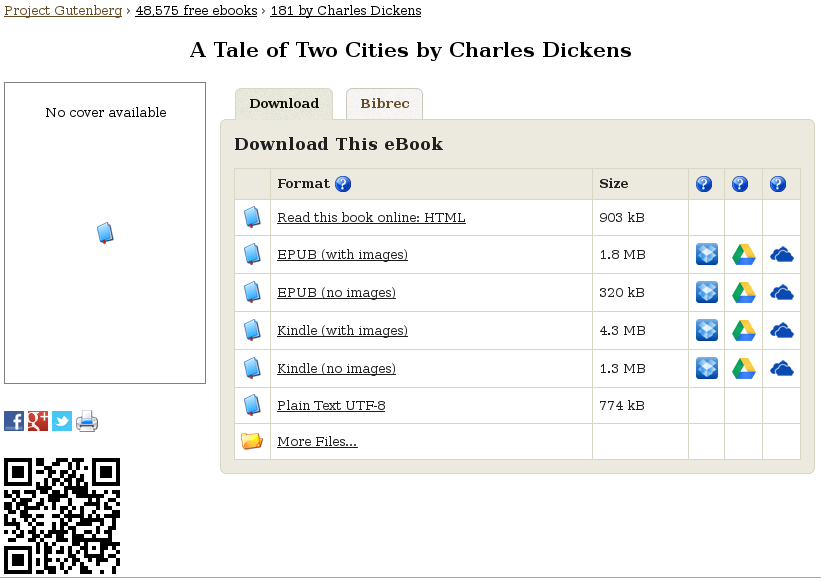
\includegraphics[width=10.cm]{figs/gutenberg-book}

\begin{flushright}
{\small
\url{http://www.gutenberg.org/ebooks/98}
}
\end{flushright}
\end{frame}

%%-----------------------------------------------------
\begin{frame}
\frametitle{No sólo en inglés}

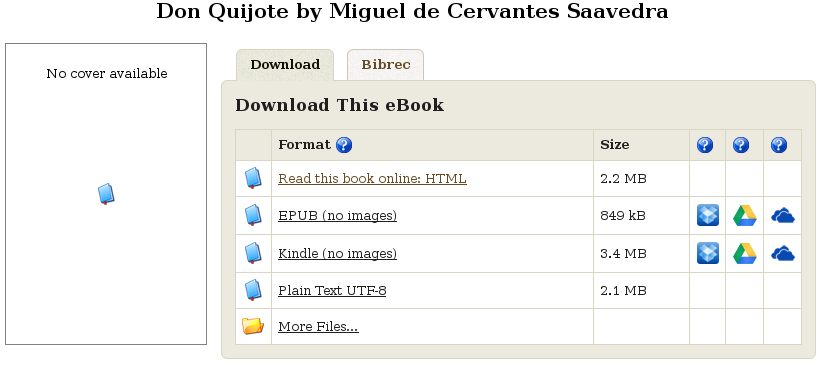
\includegraphics[width=12.cm]{figs/gutenberg-quijote}

\begin{flushright}
{\small
\url{http://www.gutenberg.org/ebooks/2000}
}
\end{flushright}
\end{frame}

%%-----------------------------------------------------
\begin{frame}
\frametitle{Proyectos relacionados}

{\Large

\begin{itemize}
\item Distributed Proofreaders \\
  \url{http://pgdp.net}
\item LibriVox: audiolibros (leidos por voluntarios) \\
  \url{http://librivox.org}
\item Wikibooks: Libros de texto ``estilo wiki''\\
  \url{http://en.wikibooks.org}
\item Cervantes Virtual: Libros en español \\
  \url{http://www.cervantesvirtual.com}
\item Europeana: artículos ``culturales'' \\
  \url{http://www.europeana.eu}
\end{itemize}

}

\end{frame}


